% Standalone source for the paper figure; build with figures/build.sh
\documentclass[border=1pt]{standalone}
% Shared preamble for the standalone figure sources.
\usepackage{times}
\usepackage{amsmath,amssymb}
\usepackage{xcolor}
\usepackage{textcomp}
\usepackage{tikz}
\usepackage{pgfplots}
\usetikzlibrary{arrows.meta,positioning,calc,fit,backgrounds}
\usepgfplotslibrary{fillbetween}
\pgfplotsset{compat=1.16}

% Colours are colour-blind safe (Okabe--Ito) and every figure also separates
% its classes by line style or fill, so the figures stay readable in greyscale.
\definecolor{cObs}{HTML}{0072B2}   % observed by the network
\definecolor{cHid}{HTML}{D55E00}   % hidden / unexplained
\definecolor{cHelp}{HTML}{009E73}  % safety helpers
\definecolor{cInk}{HTML}{333333}

\tikzset{
  box/.style={draw=cInk!70, rounded corners=1.5pt, fill=white, align=center,
              font=\scriptsize, inner sep=3pt, minimum height=0.8cm,
              line width=0.5pt},
  obs/.style={box, draw=cObs, fill=cObs!8},
  hid/.style={box, draw=cHid, fill=cHid!10},
  help/.style={box, draw=cHelp, fill=cHelp!10},
  flow/.style={-{Stealth[length=4pt]}, line width=0.6pt, draw=cInk!80},
  lbl/.style={font=\scriptsize, text=cInk!85, inner sep=1.5pt, align=center},
}
\pgfplotsset{
  every axis/.append style={font=\scriptsize, tick label style={font=\scriptsize},
                            label style={font=\scriptsize},
                            title style={font=\scriptsize\bfseries}, line width=0.5pt},
}

\begin{document}
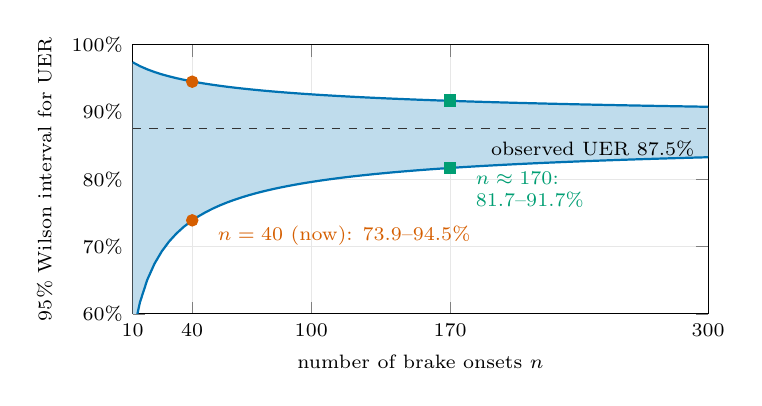
\begin{tikzpicture}
\begin{axis}[width=8.89cm, height=5.0cm, xmin=10, xmax=300,
  ymin=0.6, ymax=1.0, xlabel={number of brake onsets $n$},
  ylabel={95\% Wilson interval for UER},
  ytick={0.6,0.7,0.8,0.9,1.0}, yticklabels={60\%,70\%,80\%,90\%,100\%},
  xtick={10,40,100,170,300}, grid=major, grid style={cInk!12}]
  \addplot[name path=lo, draw=none, domain=10:300, samples=80]
    {(0.875+1.9208/x-1.96*sqrt(0.109375/x+0.9604/(x*x)))/(1+3.8416/x)};
  \addplot[name path=hi, draw=none, domain=10:300, samples=80]
    {(0.875+1.9208/x+1.96*sqrt(0.109375/x+0.9604/(x*x)))/(1+3.8416/x)};
  \addplot[cObs!25] fill between[of=lo and hi];
  \addplot[cObs, thick, domain=10:300, samples=80]
    {(0.875+1.9208/x-1.96*sqrt(0.109375/x+0.9604/(x*x)))/(1+3.8416/x)};
  \addplot[cObs, thick, domain=10:300, samples=80]
    {(0.875+1.9208/x+1.96*sqrt(0.109375/x+0.9604/(x*x)))/(1+3.8416/x)};
  \addplot[cInk, dashed, domain=10:300] {0.875};
  \addplot[only marks, mark=*, mark size=2pt, cHid] coordinates {(40,0.739)(40,0.945)};
  \addplot[only marks, mark=square*, mark size=2pt, cHelp] coordinates {(170,0.817)(170,0.917)};
  \node[font=\scriptsize, text=cHid, anchor=north west, align=left] at (axis cs:48,0.745)
    {$n=40$ (now): 73.9--94.5\%};
  \node[font=\scriptsize, text=cHelp, anchor=north west, align=left] at (axis cs:178,0.825)
    {$n\approx170$:\\81.7--91.7\%};
  \node[font=\scriptsize, anchor=north east] at (axis cs:298,0.871) {observed UER 87.5\%};
\end{axis}
\end{tikzpicture}
\end{document}
